\section[]{\textgreek{Υπάλληλοι σε ακριβώς 2 έργα}}

\begin{frame}[t, fragile, shrink]
\frametitle{Ομαδοποίηση 1:Ν με 3 πίνακες}
\begin{minipage}{\wE}
  \begin{block}{\small Να βρεθούν οι υπάλληλοι (κωδικός, όνομα, όνομα τμήματος)
     που απασχολούνται σε ακριβώς 2 έργα}
\pause \scriptsize
\en
\begin{SQL}

empid  firstname    lastname       depname
------------------------------------------------------
&mgr{  153  Μαρία        Αλεβιζάτου     Οικονομoλόγων/Λογιστών }
&mgr{  234  Αδαμαντία    Θεοτοκάτου     Γραμματείας            }
&mgr{  243  Δέσποινα     Παπαδοπούλου   Οικονομoλόγων/Λογιστών }
&mgr{  431  Κώστας       Παπαδόπουλος   Επιστημόνων/Μηχανικών  }
&mgr{  435  Αντώνης      Παύλου         Επιστημόνων/Μηχανικών  }
&mgr{  483  Ηρακλής      Μανωλάκης      Επιστημόνων/Μηχανικών  }
&mgr{  503  Μαριλένα     Κρέσπα         Οικονομoλόγων/Λογιστών }
&mgr{  835  Αθανάσιος    Πετράκης       Μάνατζμεντ/Πωλήσεων    }
\end{SQL}
\el
\end{block}
\end{minipage}
\end{frame}


\begin{frame}[t, fragile, shrink]
\frametitle{Ομαδοποίηση 1:Ν με 3 πίνακες -- Ανάλυση}
  \vspace*{-1em}
  \begin{block}{\small Ποιοι πίνακες χρειάζονται?}
    \begin{enumerate} 
      \item Στοιχεία υπαλλήλων {\ra empid, firstname, lastname},
            επομένως ο πίνακας {\sq employees}.
      \item Στοιχεία τμήματος {\ra depname},
            επομένως ο πίνακας {\sq departments}.
      \item Στοιχεία απασχόλησης: πλήθος συμμετοχών σε έργα,
            επομένως ο πίνακας {\sq workson}.
      \item Υπενθύμιση: Απασχόληση ενός υπαλλήλου σε 2 έργα σημαίνει πως
            υπάρχουν 2 εγγραφές στον πίνακα {\sq workson} με τον κωδικό του.
    \end{enumerate}
  \end{block}
  \begin{minipage}{\wE}
    \vspace*{6pt}
    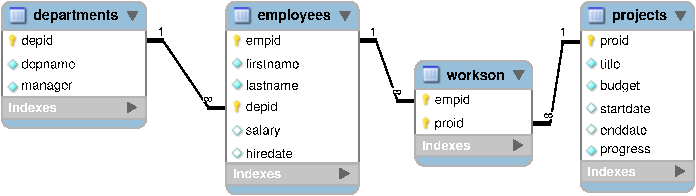
\includegraphics[scale=0.9]{../common/companyREL.pdf}
  \end{minipage}
\end{frame}



\begin{frame}[t, fragile, shrink]
\frametitle{Ομαδοποίηση 1:Ν με 3 πίνακες -- βήμα 1}
\begin{minipage}{\wE}
\vspace{-0.5cm}
  \begin{block}{\small Σύζευξη πινάκων \tdepartments\ και \temployees}
   \[
    \varrho_{d} (departments) \bowtie_{d.depid=e.depid} \varrho_{e} (employees)
   \]
\vspace{-0.5cm}
\en
\begin{SQL}
    FROM departments d INNER JOIN employees e
         ON d.depid = e.depid
\end{SQL}
\el
  \end{block}
  \pause
  \begin{block}{\small Σύζευξη \tdepartments, \temployees\ και \tworkson}
    \[
      \begin{split}
      \varrho_{d} (departments) \bowtie_{d.depid=e.depid} \varrho_{e} (employees)    \\
                                \bowtie_{e.empid=w.empid} \varrho_{w} (workson)     
      \end{split}
    \]
   \vspace{-0.5cm}
\en
\begin{SQL}
    FROM (departments d INNER JOIN employees e
                           ON d.depid = e.depid)
                        INNER JOIN workson w
                           ON e.empid = w.empid
\end{SQL}
\el
  \end{block}
\end{minipage}
\end{frame}



\begin{frame}[t, fragile, shrink]
\frametitle{Ομαδοποίηση 1:Ν με 3 πίνακες -- βήμα 2}
\begin{minipage}{\wE}
\vspace{-0.5cm}
\begin{block}{\small Ομαδοποίηση εγγραφών}
Στο ερώτημα υπάρχει ο περιορισμός για υπαλλήλους που εργάζονται σε 2 ακριβώς έργα.
Απαιτείται η ομαδοποίηση ως προς τα πεδία που ζητούνται στο ερώτημα
{\ra e.empid, e.firstname, e.lastname, d.depname}:
\[
\begin{split}
  {}_{e.empid, e.firstname, e.lastname, d.depname}  \calg_{count(*)} \\
  (
    \varrho_{d} (departments) \bowtie_{d.depid=e.depid} \varrho_{e} (employees) \\
                            \bowtie_{e.empid=w.empid} \varrho_{w} (workson)
  )
\end{split}
\]
\pause
\en
\begin{SQL}
    FROM (departments d INNER JOIN employees e
                           ON d.depid = e.depid)
                        INNER JOIN workson w
                           ON e.empid = w.empid
GROUP BY e.empid, e.firstname, e.lastname, d.depname
\end{SQL}
\el
\end{block}
\end{minipage}
\end{frame}



\begin{frame}[t, fragile, shrink]
\frametitle{Ομαδοποίηση 1:Ν με 3 πίνακες -- βήμα 3}
\begin{minipage}{\wE}
\begin{block}{\small Περιορισμός μετά την ομαδοποίηση}
Είμαστε τώρα σε θέση να εφαρμόσουμε τον περιορισμό
για ακριβώς 2 συμμετοχές υπαλλήλων σε έργα.
Στον όρο {\sq HAVING} και όχι στον όρο {\sq WHERE}:
\[
\begin{split}
  \sigma _{count(*) = 2}
  (
    {}_{e.empid, e.firstname, e.lastname, d.depname}  \calg_{count(*)} \\
    (
      \varrho_{d} (departments) \bowtie_{d.depid=e.depid} \varrho_{e} (employees) \\
                               \bowtie_{e.empid=w.empid} \varrho_{w} (workson)
    )
  )
\end{split}
\]
\pause
\vspace{-0.4cm}
\en
\begin{SQL}
    FROM (departments d INNER JOIN employees e
                           ON d.depid = e.depid)
                        INNER JOIN workson w
                           ON e.empid = w.empid
GROUP BY e.empid, e.firstname, e.lastname, d.depname
  HAVING COUNT(*) = 2
\end{SQL}
\el
  \end{block}
\end{minipage}
\end{frame}


\begin{frame}[t, fragile, shrink]
\frametitle{Ομαδοποίηση 1:Ν με 3 πίνακες -- Τελική διατύπωση}
\begin{minipage}{\wE}
\vspace{-0.5cm}
\begin{block}{\small Τελική διατύπωση: υπάλληλοι σε 2 έργα}
\[
\begin{split}
  \Pi_{e.empid, e.firstname, e.lastname, d.depname}  \\
  (
    \sigma _{count(*) = 2}
    (
      {}_{e.empid, e.firstname, e.lastname, d.depname}  \calg_{count(*)} \\
      (
        \varrho_{d} (departments) \bowtie_{d.depid=e.depid} \varrho_{e} (employees) \\
                                  \bowtie_{e.empid=w.empid} \varrho_{w} (workson)
      )
    )
  )
\end{split}
\]
\pause
\en
\begin{SQL}
  SELECT e.empid, e.firstname, e.lastname, d.depname
    FROM (departments d INNER JOIN employees e
                           ON d.depid = e.depid)
                        INNER JOIN workson w
                           ON e.empid = w.empid
GROUP BY e.empid, e.firstname, e.lastname, d.depname
  HAVING COUNT(*) = 2;
\end{SQL}
\el
  \end{block}
\end{minipage}
\end{frame}

